\documentclass{article}

\usepackage{arxiv}

\usepackage[utf8]{inputenc} % allow utf-8 input
\usepackage[T1]{fontenc}    % use 8-bit T1 fonts
\usepackage{lmodern}        % https://github.com/rstudio/rticles/issues/343
\usepackage{hyperref}       % hyperlinks
\usepackage{url}            % simple URL typesetting
\usepackage{booktabs}       % professional-quality tables
\usepackage{amsfonts}       % blackboard math symbols
\usepackage{nicefrac}       % compact symbols for 1/2, etc.
\usepackage{microtype}      % microtypography
\usepackage{graphicx}

\title{Stability of ecological and epidemiological models via
representation as Generalized Lotka-Volterra dynamics}

\author{
    Stefano Allesina
    \thanks{stefanoallesina.github.io}
   \\
    Department of Ecology \& Evolution \\
    University of Chicago \\
  Chicago, IL 60637 USA \\
  \texttt{\href{mailto:sallesina@uchicago.edu}{\nolinkurl{sallesina@uchicago.edu}}} \\
   \And
    Zachary R. Miller
   \\
    Department of Ecology \& Evolution \\
    University of Chicago \\
   \\
  \texttt{\href{mailto:zachmiller@uchicago.edu}{\nolinkurl{zachmiller@uchicago.edu}}} \\
  }



% Pandoc citation processing
\newlength{\csllabelwidth}
\setlength{\csllabelwidth}{3em}
\newlength{\cslhangindent}
\setlength{\cslhangindent}{1.5em}
% for Pandoc 2.8 to 2.10.1
\newenvironment{cslreferences}%
  {}%
  {\par}
% For Pandoc 2.11+
\newenvironment{CSLReferences}[2] % #1 hanging-ident, #2 entry spacing
 {% don't indent paragraphs
  \setlength{\parindent}{0pt}
  % turn on hanging indent if param 1 is 1
  \ifodd #1 \everypar{\setlength{\hangindent}{\cslhangindent}}\ignorespaces\fi
  % set entry spacing
  \ifnum #2 > 0
  \setlength{\parskip}{#2\baselineskip}
  \fi
 }%
 {}
\usepackage{calc} % for calculating minipage widths
\newcommand{\CSLBlock}[1]{#1\hfill\break}
\newcommand{\CSLLeftMargin}[1]{\parbox[t]{\csllabelwidth}{#1}}
\newcommand{\CSLRightInline}[1]{\parbox[t]{\linewidth - \csllabelwidth}{#1}\break}
\newcommand{\CSLIndent}[1]{\hspace{\cslhangindent}#1}

\usepackage{amsmath}
\usepackage{xcolor}
\usepackage{fancybox}
\usepackage{graphicx}


\begin{document}
\maketitle

\def\tightlist{}


\begin{abstract}
Enter the text of your abstract here.
\end{abstract}

\keywords{
    Lotka-Volterra
   \and
    Stability
   \and
    Quasi-polynomial
   \and
    Lyapunov function
  }

\hypertarget{introduction}{%
\section{Introduction}\label{introduction}}

Several models for ecological, evolutionary, and epidemiological
dynamics can be recast as a Generalized Lotka-Volterra (GLV) model via
the so-called \emph{quasi-monomial transformation}. This transformation
was discovered in the late 1980s at least three times (as far as we can
tell, independently) by different authors (Peschel and Mende 1986;
Brenig 1988; Gouzé 1990). \emph{Quasi-polynomial} (QP) systems can be
recast as a (typically, larger-dimensional) GLV in a straightforward,
mechanical manner; several other systems that do not belong to this
class can be first transformed into QP systems, and then in turn into
GLV. This shows that the Generalized Lotka-Volterra model is not only
one of the oldest models in ecology---it was originally proposed in 1920
by Lotka (Lotka 1920a, 1920b), and rediscovered by Volterra in 1926
(Volterra 1926a, 1926b)---, but a somewhat \emph{universal},
\emph{canonical} model, arising in a variety of fields and problems.

The transformation was studied, extended and applied in numerous
articles, and summarized in reviews (Rocha Filho et al. 2005; Brenig
2018) and books (Szederkényi 2012; Szederkenyi, Magyar, and Hangos
2018). Despite the wealth of literature on the subject, applications in
theoretical ecology have been so far quite limited (but see Miller and
Allesina (2021)).

The goal of this work is to provide a concise, self-contained
introduction to the transformation, illustrated by a number of examples
taken from the ecological, evolutionary and epidemiological theory, with
the hope of popularizing what is a powerful, straightforward approach.
The material requires some basic familiarity with differential equations
and linear algebra; any advanced concept is explained in detail---though
the exposition is not as formal as what found in the mathematical
literature. Throughout, we emphasize applications to the problem of
determining stability of a biological system via Lyapunov's direct
method.

While most of the material is a review or a re-elaboration of published
results, we highlight two aspects that are rarely discussed: first, we
show that stability can often be proven in a straightforward way by
considering that the perturbations of the transformed system are
constrained by the perturbations of the original system---and have
therefore a characteristic form; second, we discuss at length the (and
provide code for) numerical approaches that can be implemented to
facilitate the task of proving stability via this transformation.

We start by deriving the transformation of QP systems into GLV, using
the Leslie-Gower predator-prey model as an example; next, we analyze
FIVE? models taken from the ecological, evolutionary and epidemiological
literature, and use the transformation to prove global asymptotic
stability; we then show how non-QP systems can be turned into GLV via
auxiliary variables; we conclude by briefly presenting more advanced
techniques. The Appendix discusses numerical approaches meant to
facilitate the application of this methods to systems of interest.

\hypertarget{generalized-lotka-volterra-model}{%
\section{Generalized Lotka-Volterra
model}\label{generalized-lotka-volterra-model}}

\label{sec:glv}

The Generalized Lotka-Volterra model for \(m\) interacting populations
can be written as:

\begin{equation}
\label{eq:glv}
\dot{x}_i = x_i \left(r_i + \sum_{j=1}^m A_{ij} x_j \right)
\end{equation}

where \(\dot{x}_i\) is the derivative with respect to time of the size
(or density) of population \(i\), \(r\) is a vector of length \(m\)
containing the intrinsic growth rates (for producers) or mortality rates
(for consumers), and \(A\) is an \(m \times m\) matrix whose
coefficients \(A_{ij}\) measure the effect of population \(j\) on the
growth of population \(i\).

This set of equations admits up to \(2^m\) equilibria (i.e., choices of
\(x\) such that \(\dot{x}_i = 0\) for all \(i\)), in which some of the
populations are present at positive density (called \emph{feasible}),
and others are absent. If there is a feasible equilibrium encompassing
all populations, it is called the coexistence equilibrium, which we
indicate as \(x^\star\). If the matrix \(A\) has full rank, the
coexistence equilibrium is unique and can be computed as
\(x^\star = -A^{-1}r\). The existence of an equilibrium is necessary,
but not sufficient for coexistence in the model. For a review of the GLV
system, and closely related models, see Hofbauer and Sigmund (1998).

\hypertarget{quasi-polynomial-systems}{%
\section{Quasi-Polynomial systems}\label{quasi-polynomial-systems}}

\label{sec:qp}

We now introduce a generalization of Eq. \ref{eq:glv}, defining the
class of quasi-polynomial (QP) systems:

\begin{equation}
\label{eq:qp}
\dot{y}_i = y_i \left( s_i + \sum_{j = 1}^m M_{ij} \prod_{k = 1}^n y_k^{B_{jk}} \right)
\end{equation}

where we have \(n\) equations, \(\dot{y}_1, \ldots, \dot{y}_n\). The
vector \(s\) is of length \(n\), \(M\) is a matrix of size
\(n \times m\) containing real coefficients, and \(B\) a matrix of size
\(m \times n\), also containing real coefficients. If \(n = m\), and
thus both \(M\) and \(B\) are square matrices, and further \(B=I_n\)
(the identity matrix of size \(n\)), the model reduces to the
Generalized Lotka-Volterra model in Eq. \ref{eq:glv} with \(r = s\) and
\(A = M\). If \(B\) contains only integers, Eq. \ref{eq:qp} defines a
\emph{polynomial} system of differential equations; relaxing this
condition to allow any \(B\) composed of real numbers, we obtain a
\emph{quasi-polynomial} (QP) system.

\begin{cb}
\textbf{QP-representation of Leslie-Gower predator-prey model}

The Leslie-Gower model is simple variation on the classic Lotka-Volterra predator-prey model. We have two equations:

\begin{equation}
\label{eq:lg}
\begin{cases}
\dot{y}_1 = y_1 (\rho_1 - y_1- \alpha_1 y_2)\\
\dot{y}_2 = y_2 \left(\rho_2 - \alpha_2 \frac{y_2}{y_1} \right)
\end{cases}
\end{equation}

with $y_1$ representing the prey, $y_2$ the predator, and all coefficients are assumed to be positive. The coexistence equilibrium for the model is given by $y_1^\star = \frac{\rho_1 \alpha_2}{\rho_2 \alpha_1 + \alpha_2}$ and $y_2^\star = \frac{\rho_1 \rho_2}{\rho_2 \alpha_1 + \alpha_2}$. As we demonstrate below, the equilibrium is globally asymptotically stable---all trajectories starting at positive densities will eventually reach it.

The system differs from GLV in that we have a ratio between the predator and prey in the equation for the predator. The system is however in QP form, as seen by defining:

\begin{equation}
\label{eq:lgqp}
s = \begin{pmatrix}
\rho_1\\
\rho_2
\end{pmatrix} \quad 
M = \begin{pmatrix}
-1 & -\alpha_1 & 0\\
0 & 0 & -\alpha_2
\end{pmatrix} \quad
B = \begin{pmatrix}
1 & 0 \\
0 & 1 \\
-1 & 1
\end{pmatrix}
\end{equation}

\end{cb}

\hypertarget{from-quasi-polynomial-to-generalized-lotka-volterra}{%
\section{From Quasi-Polynomial to Generalized
Lotka-Volterra}\label{from-quasi-polynomial-to-generalized-lotka-volterra}}

\label{sec:qptoglv}

We define a set of \(m\) \emph{quasi-monomials}:

\begin{equation}
\label{eq:quasimono}
x_j = \prod_{k=1}^n y_k^{B_{jk}}
\end{equation}

A simple way to identify quasi-monomials for any system that can be
written in QP form is to consider the per capita dynamics:

\begin{equation}
\dot{\log y}_i = \frac{\dot{y}_i}{y_i} = s_i + \sum_{j = 1}^m M_{ij} \prod_{k = 1}^n y_k^{B_{jk}}
\end{equation}

As such, the set of variables, or product of powers of variables
appearing in the equations for \(\dot{\log y}_i\) defines the
quasi-monomials in \(x\).

\begin{cb}
\textbf{Quasi-monomials for the Leslie-Gower model}

For the Leslie-Gower model in Eq. \ref{eq:lg} we identify three quasi-monomials:

\begin{equation}
\label{eq:lgqm}
\begin{cases}
x_1 = y_1^1 \, y_2^0 = y_1\\
x_2 = y_1^0 \, y_2^1 = y_2\\
x_3 = y_1^{-1} \, y_2^1 = \frac{y_2}{y_1}
\end{cases}
\end{equation}

\end{cb}

\textbf{Do we need to discuss the case \(n < m\)?}

Now we show how the \(n-\)dimensional QP-system of differential
equations in Eq. \ref{eq:qp} can be recast as an \(m-\)dimensional GLV
system in Eq. \ref{eq:glv}. By chain rule, we have:

\begin{equation}
\label{eq:quasimonodt}
\begin{aligned}
\dot{x}_j &= \sum_k B_{jk}\, \dot{y}_k \, y_{k}^{(B_{jk} -1)} \prod_{l \neq k} y_{l}^{B_{jl}}\\
&=\sum_k B_{jk}\, \frac{\dot{y}_k}{y_k} \prod_{l} y_{l}^{B_{jl}}\\
&=\sum_k B_{jk}\, \frac{\dot{y}_k}{y_k} x_j\\
&=x_j \sum_k B_{jk}\, \frac{\dot{y}_k}{y_k} \\
&=x_j \left(\sum_k B_{jk} s_k + \sum_k B_{jk} \sum_l M_{kl} \prod_l y_l^{B_{kl}} \right)\\
&=x_j \left(\sum_k B_{jk} s_k + \sum_k B_{jk} \sum_l M_{kl} x_l \right)\\
&=x_j \left((B s)_j + \sum_l (B M)_{jl} x_l \right)\\
&=x_j \left(r_j + \sum_l A_{jl} x_l \right)
\end{aligned}
\end{equation}

where we have defined \(A = BM\) and \(r = B s\); \((Bs)_j\) is the
\(j^{\text{th}}\) element of the vector \(Bs\) and \((B M)_{jl}\) is the
coefficient in row \(j\) and column \(l\) of the matrix \(BM\).

\begin{cb}
\textbf{GLV representation of the Leslie-Gower model}

We can represent the Leslie-Gower model in Eq. \ref{eq:lg} as a three-dimensional GLV model defined by the quasi-monomials in Eq. \ref{eq:lgqm} and:

\begin{equation}
r = B s = \begin{pmatrix}
\rho_1\\
\rho_2\\
\rho_2 - \rho_1
\end{pmatrix}
\quad
A = B M = \begin{pmatrix}
-1 & -\alpha_1 & 0\\
0 & 0 & -\alpha_2\\
1 & \alpha_1 & -\alpha_2
\end{pmatrix}
\end{equation}

Note that $A$ is rank deficient, given that the third row can be written as the difference between the second and first row. Rank-deficiency of $A$ is expected whenever $m > n$ (as here, where we went from two to three equations).

The GLV representation of the model becomes:

\begin{equation}
\label{eq:lgglv}
\begin{cases}
\dot{x}_1 = x_1 (\rho_1 - x_1 - \alpha_1 x_2)\\
\dot{x}_2 = x_2 (\rho_2 - \alpha_2 x_3)\\
\dot{x}_3 = x_3 (\rho_2 - \rho_1 + \alpha_1 x_1 - \alpha_2 x_3)
\end{cases}
\end{equation}

\end{cb}

\hypertarget{equivalence-between-representations}{%
\section{Equivalence between
representations}\label{equivalence-between-representations}}

The original QP system and its GLV counterpart are equivalent, in the
sense that if \(y^\star\) is the coexistence equilibrium of the original
system, then there is a coexistence equilibrium for the transformed
system, calculated as \(x_i^\star = \prod_{k} (y_k^\star)^{B_{ik}}\).
Moreover, the stability of the coexistence equilibrium is unchanged.

Take the original system, with initial conditions \(y(0)\); we want to
simulate the dynamics of the original and transformed systems. Clearly,
the initial conditions of the original system are related to those of
the transformed system. We can calculate the initial conditions for the
transformed system as:

\begin{equation}
\begin{aligned}
x_i(0) &= \prod_{k} {y_k(0)}^{B_{ik}}\\
\log x_i(0) &= \sum_k B_{ik} \log y_k(0)\\
\log x_i(0) &= (B \log y_k(0))_i\\
x_i(0) &= \exp(B \log y_k(0))_i
\end{aligned}
\end{equation}

where the functions \(\log\) and \(\exp\) are applied element by element
when the argument is a vector. As such, we can compute the initial
conditions in matrix form as \(x(0) = \exp(B \log y(0))\), making sure
that the initial conditions of the transformed system are consistent
with those of the original system. Take the Leslie-Gower model: in Fig.
1 we show the dynamics of the original and transformed model, showing
that the equilibrium, trajectories and stability are consistent between
the two representations of the same dynamics.

\begin{figure}
\centering
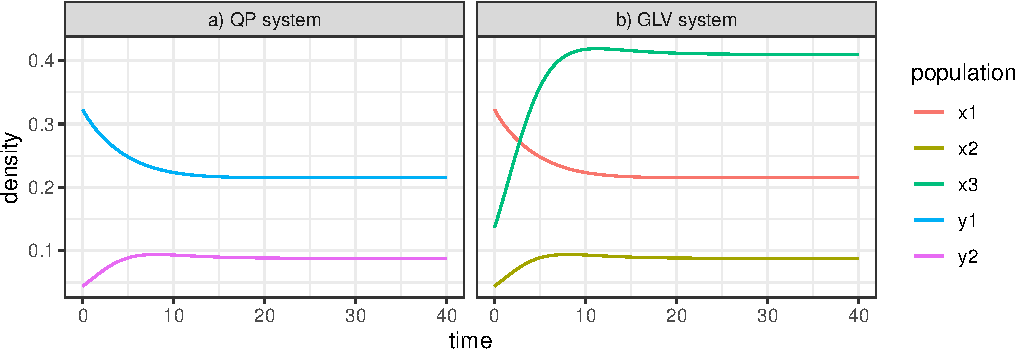
\includegraphics{GLV_embedding_files/figure-latex/fig1-1.pdf}
\caption{Dynamics for the Leslie-Gower model in its original (QP)
formulation and once transformed into a 3-dimensional GLV system. Note
that \(x_1 = y_1\) and \(x_2 = y_2\), and hence the respective
trajectories are identical. The relationship
\(x_3 = y_2 / y_1 = x_2 / x_1\) is maintained through the dynamics.}
\end{figure}

\hypertarget{stability-in-generalized-lotka-volterra}{%
\section{Stability in Generalized
Lotka-Volterra}\label{stability-in-generalized-lotka-volterra}}

\hypertarget{lyapunovs-direct-method}{%
\subsection{Lyapunov's direct method}\label{lyapunovs-direct-method}}

Provided with a dynamical system \(\dot{y}_i\)

\hypertarget{candidate-lyapunov-function-for-generalized-lotka-volterra}{%
\subsection{Candidate Lyapunov function for Generalized-Lotka
Volterra}\label{candidate-lyapunov-function-for-generalized-lotka-volterra}}

Before proceeding, we note that if Eq. \ref{eq:glv} has a feasible
(i.e., positive) coexistence equilibrium, then \(r = -A x^\star\), and
as such we can rewrite the equations more compactly as
\(\dot{x}_i = x_i \sum_{j} A_{ij} (x_j - x_j^\star) = x_i \sum_{j} A_{ij} \Delta x_j\),
where we have defined the deviation from equilibrium
\(\Delta x_j = x_j - x_j^\star\).

We now consider the candidate Lyapunov function proposed by Goh:

\begin{equation}
\label{eq:goh}
\begin{cases}
V_{x_i} = x_i - x_i^\star - x_i^\star \log \frac{x_i}{x_i^\star}\\
V = \sum_i w_i V_{x_i}
\end{cases}
\end{equation}

where each \(V_{x_i} > 0\) for any positive \(x_i \neq x_i^\star\) and
zero at the equilibrium. The weights \(w_1, \ldots w_n\) are positive.
\textbf{DISCUSS: CAN SOME WEIGHTS BE ZERO? WHAT ABOUT \(V\) unbounded}.
If we can find weights such that
\(\dot{V} = \sum_i w_i \dot{V}_{x_i} \leq 0\), we can attempt proving
stability (possibly, by invoking LaSalle's invariance principle).
Deriving:

\begin{equation}
\label{eq:gohstab}
\begin{aligned}
\dot{V} =& \sum_i w_i \left(\dot{x}_i - x_i^\star \dot{\log x_i} \right)\\
 =& \sum_i w_i \left(x_i \sum_{j} A_{ij} \Delta x_j - x_i^\star \sum_j A_{ij} \Delta x_j \right)\\
 =& \sum_i w_i \left(\Delta x_i \sum_{j} A_{ij} \Delta x_j \right)\\
 =& \sum_i \Delta x_i w_i \sum_j A_{ij} \Delta x_j\\
 =& \sum_i \sum_j w_i A_{ij} \Delta x_i \Delta x_j
\end{aligned}
\end{equation}

Note that in the sum over \(i\) and \(j\), only the symmetric part of
the matrix \(D(w) A = (w_i A_{ij})\) matters (the skew symmetric part
cancels). It is therefore convenient to define a new, symmetric matrix
\(G =\frac{1}{2} (D(w)A + A^T D(w))\), so that our expression becomes:

\begin{equation}
\label{eq:stabcond}
\dot{V} = \frac{1}{2}\sum_i \sum_j (w_i A_{ij} + A_{ji} w_j) \Delta x_i \Delta x_j = \sum_i \sum_j G_{ij} \Delta x_i \Delta x_j
\end{equation}

A symmetric matrix \(G\) satisfying
\(z^T G z = \sum_i \sum_j G_{ij} z_i z_j < 0\) for every \(z \neq 0\) is
called \emph{negative definite}. If the sum can be zero for some
\(z \neq 0\), \(G\) is called \emph{negative semi-definite}. A
symmetric, negative definite matrix has all eigenvalues real and
negative; in a negative semi-definite matrix eigenvalues can be zero. As
such, if we can identify suitable, positive (nonnegative) weights \(w\)
such that \(G\) is negative (semi-)definite, then \(\dot{V} \leq 0\) and
we can prove the stability of the equilibrium \(x^\star\).

Note that these are sufficient, but not necessary conditions for
stability---while weights that make \(G\) negative definite might not
exist, the system could still be stable, and a Lyapunov function of a
different form could prove the result.

\hypertarget{stability-in-qp-systems}{%
\subsection{Stability in QP-systems}\label{stability-in-qp-systems}}

In the Generalized Lotka-Volterra model in Eq. \ref{eq:glv}, the
variables \(x_i\) can in principle take any positive value (at least as
an initial condition), and therefore each \(\Delta x_i\) is radially
unbounded: \(\Delta x_i \in [-x_i^\star, \infty)\); moreover, we can set
(again, at least initially) each \(x_i\) to any arbitrary positive
value, irrespective of the value of the rest of the \(x_j\). In such a
setting, it is therefore difficult to prove stability via Eq.
\ref{eq:stabcond} if the matrix \(G\) is not negative (semi-)definite.

The search for weights that make \(G\) negative semi-definite (called
\emph{admissibility}) has been a focus of the literature on QP systems
as well (Figueiredo, Gleria, and Rocha Filho 2000; Gléria, Figueiredo,
and Rocha Filho 2003). Note however that, when we represent an
\(n-\)dimensional QP-system using an \(m-\)dimensional GLV system, the
quasi-monomials \(x_i\) are functions of the original variables \(y_i\).
This in turn means that the perturbations in the GLV system are a
function of the perturbations in the original system: in particular
\(\Delta x_i = \prod_{k} y_k^{B_{ik}} - \prod_{k} (y_k^\star)^{B_{ik}}\).

In practice, this means that not all perturbations \(\Delta x\) are
allowed---rather, only those compatible with the definition of the
quasi-monomials. In turn, this means that we could (and often will) find
nonnegative weights in Eq. \ref{eq:stabcond} such that
\(\dot{V} \leq 0\) and yet the matrix \(G\) \emph{is not negative
semi-definite}. In such cases, \(G\) \emph{acts} like a negative
semi-definite matrix on the \emph{admissible} perturbations, i.e., those
abiding by the form specified by the quasi-monomials.

\begin{cb}
\textbf{Stability of the Leslie-Gower model}

We consider the candidate Lyapunov function in Eq. \ref{eq:goh} for the QP-representation of the Leslie-Gower model (Eq. \ref{eq:lgglv}). A convenient choice of weights is $w = (0, \rho_1 \alpha_1 / \alpha_2 + 1, \rho_2)^T$, yielding:

\begin{equation}
G =\frac{1}{2} (D(w)A + A^T D(w)) =
\begin{pmatrix}
0 & 0 & \frac{\rho_2}{2} \\
0 & 0 & -\frac{\alpha_2}{2} \\
\frac{\rho_2}{2} & -\frac{\alpha_2}{2} & -\rho_2 \alpha_2
\end{pmatrix}
\end{equation}

We can calculate $\dot{V}$ as:

\begin{equation}
\begin{aligned}
\dot{V} &= \sum_i \sum_j G_{ij} \Delta x_i \Delta x_j\\
&= \Delta x_3 (\rho_2 \Delta x_1 - \alpha_2 \Delta x_2 - \rho_2 \alpha_2 \Delta x_3)
\end{aligned}
\end{equation}

Substituting $\Delta x_1 = y_1 - y_1^\star$, $\Delta x_2 = y_2 - y_2^\star$ and $\Delta x_3 = y_2/y_1 - y_2^\star / y_1^\star$ shows that the function $V$ does not grow in time:

\begin{equation}
\dot{V} = -\frac{(\rho_2 + y_1) (\rho_2 y_1 - \alpha_2 y_2)^2}{\alpha_2 y_1^2} \leq 0
\end{equation}

To prove stability, we need to show that the equilibrium is the only trajectory contained in the manifold (i.e., space) defined by $\dot{V} = 0$. In such case, $\rho_2 y_1 = \alpha_2 y_2$; substituting in the equation for the predator we find $\dot{y_2}|_{\dot{V} = 0} = 0$, meaning that only trajectories for which $y_2$ is constant are contained in the space defined by $\dot{V} = 0$. This in turn means that $y_1$ must also be constant, proving that the equilibrium $y^\star$ is the only trajectory contained in $\dot{V} = 0$ and therefore the global asymptotic stability of the equilibrium.
\end{cb}

\hypertarget{examples-quasi-polynomial-systems}{%
\section{Examples: quasi-polynomial
systems}\label{examples-quasi-polynomial-systems}}

In this section we present XXXX simple examples in which we prove
stability using the quasi-monomial transformation in conjunction with
the candidate Lyapunov function in Eq. \ref{eq:goh}. See Rocha Filho et
al. (2005) for other relevant examples.

\hypertarget{a-susceptible-infected-recovered-model-with-demography}{%
\subsection{A susceptible-infected-recovered model with
demography}\label{a-susceptible-infected-recovered-model-with-demography}}

\label{sec:sir}

We consider a simple S-I-R model in which mortality in all classes is
counterbalanced by the birth of susceptible individuals:

\begin{equation}
\label{eq:sir}
\begin{cases}
\begin{aligned}
\dot{y}_1 &= \delta - \delta y_1 - \beta y_1 y_2 = y_1 \left(-\delta + \delta \frac{1}{y_1} - \beta y_2 \right)\\
\dot{y}_2 &= - (\delta + \gamma) y_2 + \beta y_1 y_2 = y_2 \left(-(\delta + \gamma) + \beta y_1 \right)\\
\dot{y_3} &= \gamma y_2 - \delta y_3 = y_3 \left(-\delta + \gamma \frac{y_2}{y_3} \right)
\end{aligned}
\end{cases}
\end{equation}

where \(y_1\) represents the proportion of susceptible individuals in
the population, \(y_2\) that of the infected/infectious individuals, and
\(y_3\) the recovered individuals. The parameter \(\delta\) serves both
as a birth rate for the population, and as the mortality rate in each
compartment, \(\beta\) is the transmission rate, and \(\gamma\) the
recovery rate. We have \(y_1 + y_2 + y_3 = 1\). It is well known that if
the critical threshold
\(\mathcal R_0 = \frac{\beta}{\gamma + \delta} > 1\), the model has a
globally stable endemic equilibrium in which a constant proportion of
individuals is infected.

At the endemic equilibrium, we have \(y_1^\star = 1 / \mathcal R_0\),
\(y_2^\star = (\mathcal R_0 - 1) \delta / (\delta + \gamma)\), and
\(y_2^\star = (\mathcal R_0 - 1) \gamma / (\delta + \gamma)\), such that
the equilibrium is feasible only if \(\mathcal R_0 >1\).

We write the model as a four-dimensional GLV system, and probe the
stability of the endemic equilibrium assuming that it is positive.
First, we identify the quasi-monomials and associated matrices and
vectors:

\begin{equation}
\begin{aligned}
x = \begin{pmatrix}
y_1\\
y_2\\
\frac{1}{y_1}\\
\frac{y_2}{y_3}
\end{pmatrix}
\quad
s = \begin{pmatrix}
-\delta \\
-\delta - \gamma \\
-\delta
\end{pmatrix}
\quad
M = \begin{pmatrix}
0 & -\beta & \delta & 0\\
\beta & 0 & 0 & 0 \\
0 & 0 & 0 & \gamma
\end{pmatrix}
\quad
B = \begin{pmatrix}
1 & 0 & 0\\
0 & 1 & 0\\
-1 & 0 & 0\\
0 & 1 & -1
\end{pmatrix}
\\
r = \begin{pmatrix}
-\delta \\
-\delta - \gamma \\
\delta\\
-\gamma
\end{pmatrix}
\quad 
A = \begin{pmatrix}
0 & -\beta & \delta & 0 \\
\beta & 0 & 0 & 0\\
0 & \beta & -\delta & 0 \\
\beta & 0 & 0 & -\gamma
\end{pmatrix}
\end{aligned}
\end{equation}

Now consider the candidate Lyapunov function with weights
\(w = (1,1,0,0)^T\), and the perturbations
\(\Delta x = (y_1 - y_1^\star, y_2 - y_2^\star, 1/y_1 - 1 / y_1^\star, y_2 / y_3 - y_2^\star / y_3^\star)^T\).
Deriving with respect to time, we obtain:

\begin{equation}
\dot{V} = \frac{1}{2} \Delta x^T (D(w) A + A^T D(w)) \Delta x =  - \delta \frac{(y_1 - y_1^\star)^2}{y_1 y_1^\star} \leq 0
\end{equation}

Note that this choice of weights does not result in a negative
semi-definite matrix: the nonzero eigenvalues of \((D(w) A + A^T D(w))\)
are \(\pm \delta / 2\).

Because \(\dot{V} = 0\) whenever \(y_1 = y_1^\star\), to prove stability
we need to make sure that the equilibrium is the only trajectory
contained in the set of points satisfying \(\dot{V} = 0\). When we
evaluate \(\dot{y_2}|_{\dot{V} = 0} = 0\), meaning that \(y_2\) must be
constant for a trajectory to be contained in the space defined by
\(\dot{V} = 0\); but then inspecting the equation for \(\dot{y}_3\) is
sufficient to determine that

\hypertarget{stability-of-a-consumer-resource-model-with-inputs}{%
\subsection{Stability of a consumer-resource model with
inputs}\label{stability-of-a-consumer-resource-model-with-inputs}}

We consider a model with \(2n\) equations, equally divided into
resources (\(z_i\)) and consumers (\(y_i\)). The model can be written
as:

\begin{equation}
\label{eq:cr}
\begin{cases}
\dot{z}_i = \kappa_i - \delta_i z_i - z_i \sum_j C_{ij} y_j\\
\dot{y}_i = - \mu_i y_i + y_i \epsilon_i \sum_j C_{ji} z_j
\end{cases}
\end{equation}

where \(\kappa_i\) is the input to resource \(i\), \(\delta_i\) its
degradation rate, \(C_{ij}\) the consumption of \(i\) by consumer \(j\),
\(\mu_i\) the mortality rate of consumer \(i\), and \(\epsilon_i\) the
efficiency of transformation of resources into consumers. We want to
show that, whenever a feasible equilibrium exists, it is globally
stable.

We identify \(3n\) quasi-monomials: \(x_i = z_i\) for
\(i \in \{1, \ldots, n\}\), \(x_i = y_i\) for
\(i \in \{n + 1, \ldots, 2 n\}\), and finally \(x_i = 1 / z_i\) for
\(i \in \{2 n + 1, \ldots, 3 n\}\). This allows us to rewrite the system
in Eq. \ref{eq:cr} as a QP-system defined by:

\begin{equation}
\label{eq:crqp}
s = \begin{pmatrix}
-\delta \\
-\mu \\
\end{pmatrix} \quad 
M = \begin{pmatrix}
0_{n \times n} & -C & D(\kappa)\\
D(\epsilon)C^T & 0_{n \times n} & 0_{n \times n}
\end{pmatrix} \quad
B = \begin{pmatrix}
I_n & 0_{n \times n}\\
0_{n \times n} & I_n\\
-I_n & 0_{n \times n}
\end{pmatrix}
\end{equation}

where \(0_{n \times n}\) is a matrix of size \(n \times n\) containing
zeros, \(I_n\) is the identity matrix of size \(n\) and \(D(\theta)\)
the diagonal matrix with \(\theta\) on the diagonal. We rewrite the
system as a \(3n-\)dimensional GLV defined by:

\begin{equation}
r = B s = \begin{pmatrix}
-\delta \\
-\mu \\
\delta
\end{pmatrix} \quad
A = B M = \begin{pmatrix}
0_{n \times n} & -C & D(\kappa)\\
D(\epsilon) C^T & 0_{n \times n} & 0_{n \times n}\\
0_{n \times n} & C & -D(\kappa)
\end{pmatrix}
\end{equation}

We now consider the candidate Lyapunov function in Eq. \ref{eq:goh} with
weights \(w = (1_n, 1 / \epsilon, 0_n)\). Our matrix \(G\) becomes:

\begin{equation}
G = \frac{1}{2}(D(w) A + A^T D(w)) = \begin{pmatrix}
0_{n \times n} & 0_{n \times n} & \frac{1}{2} D(\kappa)\\
0_{n \times n} & 0_{n \times n} & 0_{n \times n}\\
\frac{1}{2} D(\kappa) & 0_{n \times n} & 0_{n \times n}
\end{pmatrix}
\end{equation}

The matrix is clearly non negative semi-definite. And yet, when we
consider the perturbations:
\(\Delta x = (z - z^\star, y - y^\star, 1 / z - 1 / z^\star)^T\), the
derivative with respect to time in Eq. \ref{eq:stabcond} reduces to:

\begin{equation}
\dot{V} = \sum_i k_i (z_i - z_i^\star) \left( \frac{1}{z_i} - \frac{1}{z_i^\star} \right) = - \sum_i \frac{k_i}{z_i z_i^\star} (z_i - z_i^\star)^2 \leq 0
\end{equation}

Note that when \(\dot{V} = 0\) the resources are all at equilibrium; but
this implies that the consumers must also be at equilibrium, because all
\(\dot{y}_i|_{\dot{V} = 0} = \dot{y}_i|_{z = z^\star} = 0\).

\hypertarget{reducing-nonlinearities-in-a-model-with-higher-order-interactions}{%
\subsection{Reducing nonlinearities in a model with higher-order
interactions}\label{reducing-nonlinearities-in-a-model-with-higher-order-interactions}}

\label{sec:hoi}

The last few years have seen a resurgence in the interest for so-called
higher-order interactions. When including interactions of more than two
populations at a time, dynamics can be altered dramatically. For
example, Grilli \textit{et al.} showed stabilization for the replicator
equation when three or more players interact. The simplest model is that
for a replicator equation describing a three-player game of
rock-paper-scissors:

\begin{equation}
\label{eq:rpshoi}
\begin{cases}
\dot{y}_1 = y_1 (2 y_3^2 + y_1 y_3 - 2 y_1 y_2 - y_2^2)\\
\dot{y}_2 = y_2 (2 y_1^2 + y_1 y_2 - 2 y_2 y_3 - y_3^2)\\
\dot{y}_3 = y_3 (2 y_2^2 + y_2 y_3 - 2 y_1 y_3 - y_2^2)
\end{cases}
\end{equation}

with dynamics occurring on the simplex \(y_1 + y_2 + y_3 = 1\). The
system has a single feasible equilibrium
\(y_i^\star = \frac{1}{3} \quad \forall i\). Note that the system is in
QP-form as defined by the monomials:

\begin{equation}
\label{eq:rpshoimon}
x = 
\begin{pmatrix}
y_1^2\\ y_2^2 \\ y_3^2 \\ y_1 y_2 \\ y_1 y_3 \\ y_2 y_3
\end{pmatrix} 
\end{equation}

and parameters

\begin{equation}
\label{eq:rpshoiqp}
\lambda = \begin{pmatrix}
0\\
0\\
0
\end{pmatrix} \quad 
M = \begin{pmatrix}
0 & -1 & 2 & -2 & 1 & 0\\
2 & 0 & -1 & 1 & 0 & -2\\
-1 & 2 & 0 & 0 & -2 & 1
\end{pmatrix} \quad
B = \begin{pmatrix}
2 & 0 & 0 \\
0 & 2 & 0 \\
0 & 0 & 2 \\
1 & 1 & 0 \\
1 & 0 & 1 \\
0 & 1 & 1
\end{pmatrix}
\end{equation}

As such, the model in Eq. \ref{eq:rpshoi} with three variables
(equivalent to two equations, given the constrain of dynamics happening
in the simplex) and higher-order interactions can be recast as a GLV
model with six variables, and parameters:

\begin{equation}
r = B \lambda = \vec{0}
\quad
A = B M = \begin{pmatrix}
0 & -2 & 4 & -4 & 2 & 0 \\ 
4 & 0 & -2 & 2 & 0 & -4 \\ 
-2 & 4 & 0 & 0 & -4 & 2 \\ 
2 & -1 & 1 & -1 & 1 & -2 \\ 
-1 & 1 & 2 & -2 & -1 & 1 \\ 
1 & 2 & -1 & 1 & -2 & -1
\end{pmatrix}
\end{equation}

Note that matrix \(A\) has eigenvalues
\(-\frac{3}{2}(1 \pm 3 \sqrt{3})\) and an additional four eigenvalues
equal to zero (i.e., it has rank 2, the number of independent equations
in the original system).

By choosing the candidate Lyapunov in Eq. \ref{eq:goh} function with
weights \(\gamma = (1,1,1, 2,2,2)^T\) and considering the perturbations
\(\Delta x = (y_1^2 - {y_1^\star}^2, y_2^2 - {y_2^\star}^2, y_3^2 - {y_3^\star}^2, y_1 y_2 - y_1^\star y_2^\star, y_1 y_3 - y_1^\star y_3^\star, y_2 y_3 - y_2^\star y_3^\star)^T\),
we obtain:

\begin{equation}
\begin{aligned}
\dot{V} &= -\frac{2}{3} \left(y_1^2 + y_2^2 + y_3^2 - y_1 y_2 -y_1 y_3 - y_2 y_3 \right) \\
&=-\frac{1}{3} \left((y_1 - y_2)^2 + (y_1 - y_3)^2 + (y_2 - y_3)^2\right) \leq 0
\end{aligned}
\end{equation}

The derivative is thus negative for any \(y\) but the equilibrium point,
proving the stability of the equilibrium.

\hypertarget{examples-non-quasi-polynomial-systems}{%
\section{Examples: non quasi-polynomial
systems}\label{examples-non-quasi-polynomial-systems}}

\hypertarget{further-transformations}{%
\section{Further transformations}\label{further-transformations}}

\hypertarget{other-approaches-to-stability-for-lotka-volterra}{%
\section{Other approaches to stability for
Lotka-Volterra}\label{other-approaches-to-stability-for-lotka-volterra}}

\hypertarget{conclusions}{%
\section*{Conclusions}\label{conclusions}}
\addcontentsline{toc}{section}{Conclusions}

\hypertarget{refs}{}
\begin{CSLReferences}{1}{0}
\leavevmode\hypertarget{ref-brenig1988complete}{}%
Brenig, Léon. 1988. {``Complete Factorisation and Analytic Solutions of
Generalized Lotka-Volterra Equations.''} \emph{Physics Letters A} 133
(7-8): 378--82.

\leavevmode\hypertarget{ref-brenig2018reducing}{}%
---------. 2018. {``Reducing Nonlinear Dynamical Systems to Canonical
Forms.''} \emph{Philosophical Transactions of the Royal Society A:
Mathematical, Physical and Engineering Sciences} 376 (2124): 20170384.

\leavevmode\hypertarget{ref-figueiredo2000boundedness}{}%
Figueiredo, A, IM Gleria, and TM Rocha Filho. 2000. {``Boundedness of
Solutions and Lyapunov Functions in Quasi-Polynomial Systems.''}
\emph{Physics Letters A} 268 (4-6): 335--41.

\leavevmode\hypertarget{ref-gleria2003numerical}{}%
Gléria, IM, A Figueiredo, and TM Rocha Filho. 2003. {``A Numerical
Method for the Stability Analysis of Quasi-Polynomial Vector Fields.''}
\emph{Nonlinear Analysis: Theory, Methods \& Applications} 52 (1):
329--42.

\leavevmode\hypertarget{ref-gouze1990transformation}{}%
Gouzé, Jean-Luc. 1990. {``Transformation of Polynomial Differential
Systems in the Positive Orthant.''} PhD thesis, INRIA.

\leavevmode\hypertarget{ref-hofbauer1998evolutionary}{}%
Hofbauer, Josef, and Karl Sigmund. 1998. \emph{Evolutionary Games and
Population Dynamics}. Cambridge university press.

\leavevmode\hypertarget{ref-lotka1920analytical}{}%
Lotka, Alfred J. 1920a. {``Analytical Note on Certain Rhythmic Relations
in Organic Systems.''} \emph{Proceedings of the National Academy of
Sciences} 6 (7): 410--15.

\leavevmode\hypertarget{ref-lotka1920undamped}{}%
---------. 1920b. {``Undamped Oscillations Derived from the Law of Mass
Action.''} \emph{Journal of the American Chemical Society} 42 (8):
1595--99.

\leavevmode\hypertarget{ref-miller2021metapopulations}{}%
Miller, Zachary R, and Stefano Allesina. 2021. {``Metapopulations with
Habitat Modification.''} \emph{bioRxiv}.

\leavevmode\hypertarget{ref-peschel1986predator}{}%
Peschel, Manfred, and Werner Mende. 1986. \emph{The Predator-Prey Model:
Do We Live in a Volterra World?} Springer.

\leavevmode\hypertarget{ref-rocha2005lotka}{}%
Rocha Filho, Tarcísio M, Iram M Gléria, Annibal Figueiredo, and Léon
Brenig. 2005. {``The Lotka--Volterra Canonical Format.''}
\emph{Ecological Modelling} 183 (1): 95--106.

\leavevmode\hypertarget{ref-szederkenyi2018analysis}{}%
Szederkenyi, Gabor, Attila Magyar, and Katalin M Hangos. 2018.
\emph{Analysis and Control of Polynomial Dynamic Models with Biological
Applications}. Academic Press.

\leavevmode\hypertarget{ref-szederkenyi2012computational}{}%
Szederkényi, Gábor. 2012. {``Computational Methods for the Analysis of
Nonnegative Polynomial Systems.''} PhD thesis, MTA SZTAKI.

\leavevmode\hypertarget{ref-volterra1926fluctuations}{}%
Volterra, Vito. 1926a. {``Fluctuations in the Abundance of a Species
Considered Mathematically.''} \emph{Nature} 118 (2972): 558--60.

\leavevmode\hypertarget{ref-volterra1926variazioni}{}%
---------. 1926b. {``Variazioni e Fluttuazioni Del Numero d'individui in
Specie Animali Conviventi.''} \emph{Memorie Della Regia Accademia
Nazionale Dei Lincei} 2: 31--113.

\end{CSLReferences}

\bibliographystyle{abbrv}
\bibliography{references.bib}


\end{document}
